\documentclass[smaller]{beamer}
\usetheme[english]{Berlin}
\usepackage{ngerman}
\useoutertheme{infolines}
\beamertemplatenavigationsymbolsempty
\usepackage{pgfplots,tikz,subfigure}
\usepackage{amsmath,amsthm}
\usepackage{hyperref,graphics,graphicx,color,algorithm,algorithmic,enumerate}
\usepackage{mymacros,wrapfig,relsize}
\usepackage{pict2e}
\usepackage[utf8x]{inputenc}

\newcommand{\ri}{\mathrm{i}}
\newcommand{\T}{\mathsf{T}}
\renewcommand{\H}{\mathsf{H}}
\newcommand{\eps}{\varepsilon}
\newcommand{\To}{\rightarrow}
\newcommand{\sddots}{\scalebox{0.6}{$\ddots$}}
\usepackage[pdf]{pstricks}
\usepackage{sansmathfonts}
%\usepackage{arev}
%\renewcommand\familydefault{\sfdefault}

\DeclareMathOperator{\loc}{loc}
\DeclareMathOperator{\rank}{rank}
\DeclareMathOperator{\RE}{Re}
\DeclareMathOperator{\IM}{Im}
\DeclareMathOperator{\In}{In}
\DeclareMathOperator{\im}{im}
\DeclareMathOperator{\Gl}{Gl}
\DeclareMathOperator{\spa}{span}
\DeclareMathOperator{\ext}{{ext}}
\DeclareMathOperator{\ind}{ind}
\DeclareMathOperator{\normalrank}{normalrank}
\DeclareMathOperator{\essup}{ess\,sup}
\DeclareMathOperator{\vect}{vec}

\newcommand{\re}{\mathrm{e}}
\newcommand{\ddt}{\tfrac{\mathrm{d}}{\mathrm{d}t}}
\newcommand{\sys}[4]{\left[\begin{array}{c|c} #1 & #2 \\ \hline #3 & #4 \end{array}\right]}

\renewcommand{\tilde}{\widetilde}
\renewcommand{\hat}{\widehat}

\title[]{Optimierung f\"ur Studierende der Informatik}
\subtitle{-- 1. Vorlesung --}
\author[Matthias Voigt]{\textbf{Matthias Voigt$^{1,2}$}}
\institute[]{
\begin{columns}
%\begin{center}
\column{0.45\textwidth}{\centering {$^1$Universit\"at Hamburg \\ Fachbereich Mathematik \\ Hamburg \\ }}
\column{0.45\textwidth}{\centering {$^2$Technische Universit\"at Berlin \\ Institut f\"ur Mathematik \\ Berlin  \\}}
%\end{center}
\end{columns}
}
\date[]{Universit\"at Hamburg
\begin{columns}
\column{0.45\textwidth}{\centering 
\includegraphics[width = 1.2\textwidth]{uhh-logo.png}\\}
\end{columns}
}

\definecolor{tucgreen}{rgb}{0.0,0.5,0.27}
\definecolor{tucred}{rgb}{0.75,0,0}
\definecolor{tucorange}{rgb}{1.0,.5625,0}
\definecolor{mpired}{HTML}{990000}
\definecolor{mpigreen}{HTML}{5C871D}
\definecolor{mpiblue}{HTML}{006AA9}
\definecolor{mpibg1}{HTML}{5D8B8A}
\definecolor{mpibg2}{HTML}{BFDFDE}
\definecolor{mpibg3}{HTML}{A7C1C0}
\definecolor{mpibg4}{HTML}{7DA9A8}
\definecolor{mpigrey}{rgb}{0.9294,0.9294,0.8784}

\begin{document}

\maketitle

%\section{Motivating Example}
%\frame{\tableofcontents}
%\frame{\tableofcontents[currentsection,currentsubsection]}

\begin{frame}
\frametitle{Ein Di\"atproblem}
Paul möchte sich möglichst preiswert ernähren, allerdings so, dass er pro Tag mindestens 2000kcal, 55g Proteine und 800mg Kalzium erhält. Er wählt sechs Lebensmittel aus, die günstig zu erstehen sind:
\begin{enumerate}[1.]
\item \textbf{Haferflocken:} Eine 28g Packung liefert 110kcal, 4g Protein, 2mg Kalzium    
und kostet 25 Cent.
\item \textbf{Huhn:} 100g liefern 205kcal, 32g Protein und 12mg Kalzium; Preis: 130 Cent.
\item \textbf{Eier:} Eine Doppelpackung liefert 160kcal, 13g Protein und 54mg Kalzium; bezahlen muss man 85 Cent pro Doppelpack.
\item \textbf{Milch:} Eine kleine Packung liefert 160kcal, 8g Protein und 285mg Kalzium; Preis: 70 Cent.
\item \textbf{Kirschkuchen:} Ein Stück (170g) liefert 420kcal, 4g Protein und 22mg Kalzium; Preis: 95 Cent.
\item \textbf{Bohnen:} Eine Packung (260g) liefert 260kcal, 14g Protein und 80mg Kalzium; Preis: 98 Cent.
\end{enumerate}
\end{frame}

\begin{frame}
\frametitle{Ein Di\"atproblem}
\begin{table}
\caption{Alle Daten auf einen Blick}
\begin{tabular}{c|cccc}
      & Energie (kcal) &  Protein (g) &  Kalzium (mg) &  Preis (Cent)  \\ \hline
Haferflocken  &  110  &   4  &  2  &  25 \\
Huhn  &  205  &  32   &  12  & 130 \\
Eier  &  160  &  13   &  54  &  85 \\
Milch   &  160   &   8   & 285   &  70 \\
Kirschkuchen  &   420   & 4   & 22  &   95 \\
Bohnen   & 260  &  14  & 80  &  98
\end{tabular}
\end{table}
\vspace*{0.2cm}
Paul denkt über seine Mahlzeiten nach: Beispielsweise würden 
10 Portionen Bohnen alles Erforderliche an Energie, Protein und Kalzium liefern – zu einem Preis von nur (?) 980 Cent pro Tag. 

Mehr als 2 Portionen Bohnen pro Tag ist aber zu viel; er legt Obergrenzen fest:
\end{frame}

\begin{frame}
 \frametitle{Ein Diätproblem}
  \begin{enumerate}
  \item \textbf{Haferflocken:} höchstens 4 Portionen pro Tag;
  \item \textbf{Huhn:} höchstens 3 Portionen pro Tag;
  \item \textbf{Eier:} höchstens 2 Portionen pro Tag;
  \item \textbf{Milch:} höchstens 8 Portionen pro Tag;
  \item \textbf{Kirschkuchen:} höchstens 2 Portionen pro Tag;
  \item \textbf{Bohnen:} höchstens 2 Portionen pro Tag.
  \end{enumerate}
  \vspace*{0.2cm}
  Ein Blick auf die Daten lässt erkennen: 8 Portionen Milch und 2 Portionen Kirschkuchen pro Tag liefern alles Nötige für nur 750 Cent. 

  Man könnte auch etwas weniger Kuchen nehmen oder etwas weniger Milch – oder eine andere Kombination ausprobieren: \structure{trial and error} nennt man das. \alert{Hilft das weiter?}
\end{frame}

\begin{frame}
 \frametitle{Systematische Herangehensweise}
 Um systematisch vorzugehen, führen wir für jedes Lebensmittel eine Variable ein: 
 \begin{itemize}
  \item $x_1$ bezeichnet die Anzahl der Portionen von Haferflocken pro Tag, 
  \item $x_2$ die Anzahl der Huhn-Portionen pro Tag,
  \item $x_3$ die Anzahl der Ei-Portionen pro Tag etc. 
 \end{itemize}
 Beispielsweise bedeutet $x_6 = 1.5$, dass Paul 1.5 Portionen Bohnen pro Tag zu sich nimmt.

 Wir formulieren das vorgestellte Problem auf folgende Art:
\end{frame}

\begin{frame}
 \frametitle{LP-Probleme}
 \begin{align*}
\begin{alignedat}{8}
& \text{minimiere } & 25x_1 &\ + &\ 130x_2 &\ + &\ 85x_3 &\ + &\ 70x_4 &\ + &\ 95x_5 &\ + &\ 98x_6 & & \\
& \rlap{unter den Nebenbedingungen} & & & & & & & & & & & & & \\
&& 110x_1 &\ + &\ 205x_2 &\ + &\ 160x_3 &\ + &\ 160x_4 &\ + &\ 420x_5 &\ + &\ 260x_6 &\ \geq &\  2000,\ \\
&&   4x_1 &\ + &\ 32x_2 &\ + &\ 13x_3 &\ + &\ 8x_4 &\ + &\ 4x_5 &\ + &\ 14x_6 &\ \geq &\  55,\ \\
&&   2x_1 &\ + &\ 12x_2 &\ + &\ 54x_3 &\ + &\ 285x_4 &\ + &\ 22x_5 &\ + &\ 80x_6 &\ \geq &\  800,\ \\
&& & & & & & & & & & & \llap{$0\ \leq\ x_1$} &\ \leq &\ 4,\ \\
&& & & & & & & & & & & \llap{$0\ \leq\ x_2$} &\ \leq &\ 3,\ \\
&& & & & & & & & & & & \llap{$0\ \leq\ x_3$} &\ \leq &\ 2,\ \\
&& & & & & & & & & & & \llap{$0\ \leq\ x_4$} &\ \leq &\ 8,\ \\
&& & & & & & & & & & & \llap{$0\ \leq\ x_5$} &\ \leq &\ 2,\ \\
&& & & & & & & & & & & \llap{$0\ \leq\ x_6$} &\ \leq &\ 2.\ 
\end{alignedat}
\end{align*}
Probleme dieser Art werden \structure{lineare Programmierungsprobleme (oder lineare Optimierungsprobleme)} genannt; kurz: \structure{LP-Probleme}. 
\end{frame}

\begin{frame}
 \frametitle{Weitere Beispiele}
 \begin{align} \label{eq:1.1}
\begin{alignedat}{5}
& \text{maximiere } & 5x_1 &\ + &\ 4x_2 &\ + &\ 3x_3 & & \\
& \rlap{unter den Nebenbedingungen} & & & & & & & \\
&& 2x_1 &\ + &\ 3x_2 &\ + &\  x_3 &\ \leq &\  5,\ \\
&& 4x_1 &\ + &\  x_2 &\ + &\ 2x_3 &\ \leq &\ 11,\ \\
&& 3x_1 &\ + &\ 4x_2 &\ + &\ 2x_3 &\ \leq &\  8,\ \\
&& & & & & \llap{$x_1, x_2, x_3$} &\ \geq &\  0,\
\end{alignedat}
\end{align}

\begin{align} \label{eq:1.2}
\begin{alignedat}{6}
& \text{minimiere } & 3x_1 &\ - &\ x_2 & & & & & & \\
& \rlap{unter den Nebenbedingungen} & & & & & & & &  \\
&& -x_1 &\ + &\ 6x_2 &\ - &\  x_3 &\ + &\  x_4 &\ \geq &\ -3,\ \\
&&      &\   &\ 7x_2 &\   &\      &\ + &\ 2x_4 &\ =    &\  5,\ \\
&&  x_1 &\ + &\  x_2 &\ + &\  x_3 &\   &\      &\ =    &\  1,\ \\
&&      &\   &\      &\   &\  x_3 &\ + &\  x_4 &\ \leq &\  2,\ \\
&& & & & & & & \llap{$x_2, x_3$} &\ \geq &\  0.\
\end{alignedat}
\end{align}
\end{frame}

\begin{frame}
\frametitle{Lineare Nebenbedingungen}
\textbf{Definition:} Eine Funktion $f: \R^n \rightarrow \R$ wird \structure{lineare Funktion} genannt, falls
\begin{equation}
\label{eq:1:3}
f ( x_1,\ldots,x_n ) = c_1x_1 + \ldots + c_nx_n
\end{equation}
für reelle Zahlen $c_1, \ldots, c_n$ gilt. 

Mit dem Summenzeichen geschrieben lautet die Gleichung \eqref{eq:1:3}:
\begin{equation*}
f(x_1,\ldots,x_n) = \sum_{j=1}^{n}{c_jx_j}.
\end{equation*}

Ist $b$ eine reelle Zahl, so nennt man 
\begin{equation}
\label{eq:1:4}
c_1x_1 + \ldots + c_nx_n = b
\end{equation}
eine \structure{lineare Gleichung}. Wir betrachten auch \structure{lineare Ungleichungen}:
\begin{align}
\label{eq:1:5}
c_1x_1 + \ldots + c_nx_n &\leq b, \\
\label{eq:1:6}
c_1x_1 + \ldots + c_nx_n &\geq b.
\end{align}
Gleichungen bzw. Ungleichungen der Arten \eqref{eq:1:4}, \eqref{eq:1:5} und \eqref{eq:1:6} werden von uns \structure{lineare Nebenbedingungen} oder einfach nur \structure{Nebenbedingungen} genannt.
\end{frame}

\begin{frame}
\frametitle{LP-Probleme in Standardform}
 Unter einem linearen Programmierungsproblem (kurz: LP-Problem) verstehen wir das Problem, eine lineare Funktion unter einer endlichen Anzahl von linearen Nebenbedingungen zu minimieren oder zu maximieren. (Man sagt auch {\glqq}lineares Optimierungsproblem{\grqq}.)
 
Wir beschränken uns auf \structure{LP-Probleme in Standarform}:
\begin{align} \label{eq:1.7}
\begin{alignedat}{5}
& \text{maximiere } & c_1x_1 &\ + &\ \ldots &\ + &\ c_nx_n & & \\
& \rlap{unter den Nebenbedingungen} & & & & & & & \\
&& a_{11}x_1 &\ + &\ \ldots &\ + &\ a_{1n}x_n &\ \leq &\ b_1,\ \\
&& & & & \ \ \vdots & & &  \\
&& a_{m1}x_1 &\ + &\ \ldots &\ + &\ a_{mn}x_n &\ \leq &\ b_m,\ \\
&& & & & & \llap{$x_1, \ldots, x_n$} &\ \geq &\ 0.\ 
\end{alignedat}
\end{align}
\end{frame}

\begin{frame}
 \frametitle{Zul\"assige und optimale L\"osungen}
 \begin{itemize}
 \item Die Funktion eines LP-Problems, die zu minimieren bzw. zu maximieren ist, wird \structure{Zielfunktion} genannt. 

 \item In \eqref{eq:1.1} ist also $5x_1 + 4x_2 + 3x_3$ die Zielfunktion, während in \eqref{eq:1.2} die Zielfunktion $3x_1 − x_2$ lautet. 

 \item Eine Belegung der Variablen $x_1,\ldots, x_n$, die alle Nebenbedingungen eines LP-Problems erfüllt, nennt man eine \structure{zulässige Lösung}.

 \item Eine zulässige Lösung, für die die Zielfunktion maximal bzw. minimal ist (je nach Art des LP-Problems), nennt man eine \structure{optimale Lösung}. 
  
 \item Den zu einer optimalen Lösung $(x_1, \ldots, x_n)$ gehörigen Zielfunktionswert nennt man den \structure{optimalen Zielfunktionswert}.
 \end{itemize}
\end{frame}

\begin{frame}
 \frametitle{Unl\"osbare Probleme}
 Es gibt LP-Probleme, die keine zulässige Lösung besitzen; solche LP-Probleme nennt man \structure{unlösbar}. 
 
 Hier ein Beispiel:
\begin{align*}
\begin{alignedat}{4}
& \text{maximiere } & 3x_1 &\ - &\ x_2 & & \\
& \rlap{unter den Nebenbedingungen} & & & & & \\
&&   x_1 &\ + &\  x_2 &\ \leq &\   2,\ \\
&& -2x_1 &\ - &\ 2x_2 &\ \leq &\ -10,\ \\
&& & & \llap{$x_1, x_2$} &\ \geq &\ 0.\ 
\end{alignedat}
\end{align*}
\end{frame}

\begin{frame}
 \frametitle{Unbeschr\"ankte Probleme}
 Es gibt auch LP-Probleme, die zwar zulässige Lösungen besitzen, aber keine ihrer zulässigen Lösungen ist optimal. Hier ein Beispiel:
\begin{align*}
\begin{alignedat}{4}
& \text{maximiere } & x_1 &\ - &\ x_2 & & \\
& \rlap{unter den Nebenbedingungen} & & & & & \\
&& -2x_1 &\ + &\  x_2 &\ \leq &\ -1,\ \\
&&  -x_1 &\ - &\ 2x_2 &\ \leq &\ -2,\ \\
&& & & \llap{$x_1, x_2$} &\ \geq &\ 0.\ 
\end{alignedat}
\end{align*}

In diesem Beispiel gibt es zu jeder Zahl $M$ eine zulässige Lösung $x_1,x_2$ mit $x_1-x_2 > M$. Derartige Probleme nennt man \structure{unbeschränkt}.
\end{frame}

\begin{frame}
 \frametitle{Matrixschreibweise}
 In Matrixschreibweise lässt sich \eqref{eq:1.7} besonders kompakt darstellen:
\begin{align}
%\tag{\ref*{eq:1.7}'}
\begin{alignedat}{3}
\label{eq:1:7'}
& \text{maximiere } & c^\T x & & \\
& \rlap{unter den Nebenbedingungen} & & & \\
&& Ax &\ \leq &\ b,\ \\
&&  x &\ \geq &\ 0.\
\end{alignedat}
\end{align}
 Hier ist:
 \begin{itemize}
  \item $A = \begin{pmatrix} a_{11} & \ldots & a_{1n} \\ \vdots & \ddots & \vdots \\ a_{m1} & \ldots & a_{mn} \end{pmatrix}$,
  \item $c^\T = (c_1, \ldots, c_n)$, $x= \begin{pmatrix} x_1 \\ \vdots \\ x_n \end{pmatrix}$, $b = \begin{pmatrix} b_1 \\ \vdots \\ b_m \end{pmatrix}$,
  \item $0$ bezeichnet den Nullvektor der Länge $n$; die beiden Ungleichungen sind komponentenweise zu verstehen.
 \end{itemize}
\end{frame}

\begin{frame}
 \frametitle{Einige Sprechweisen}
 Einige Sprechweisen:
 \begin{itemize}
  \item Häufig wird auch einfach \structure{{\glqq}lineares Programm{\grqq}} anstelle von {\glqq}lineares Programmierungsproblem{\grqq} ({\glqq}LP-Problem\grqq) gesagt.
  \item Die Menge aller zulässigen Lösungen eines LP-Problems nennt man   
    auch den \structure{zulässigen Bereich}.
  \item Kommt eine Variable bei den Nichtnegativitätsbedingungen nicht vor, so 
    spricht man von einer \structure{freien Variablen}. 
 \end{itemize}
 Beispielsweise sind in \eqref{eq:1.2} $x_1$ und $x_4$ freie Variablen.
\end{frame}

\begin{frame}
 \frametitle{\"Uberf\"uhrung in Standardform}
 Man kann jedes LP-Problem durch sehr einfache, \alert{kleine {\glqq}Tricks{\grqq}} in Standardform überführen:
 \begin{itemize}
 \item Minimiere $3x_1 - 4x_2 + 5x_3$ $\quad\Leftrightarrow\quad$ maximiere $- 3x_1 + 4x_2 - 5x_3$,
 \item Nebenbedingung $a_1x_1 + \ldots + a_nx_n \ge b$ $\quad\Leftrightarrow\quad$ $-a_1x_1 - \ldots - a_nx_n \le -b$, 
 \item Nebenbedingung $a_1x_1 + \ldots + a_nx_n = b$ $\quad\Leftrightarrow\quad$ Nebenbedingungen
  \begin{align*}
         a_1x_1 + \ldots + a_nx_n &\le b, \\
          -a_1x_1 - \ldots - a_nx_n &\le -b.
   \end{align*}
  \end{itemize}
\end{frame}

\begin{frame}
 \frametitle{\"Uberf\"uhrung in Standardform}
 \begin{itemize}
 \item Und was kann man machen, wenn man es mit einer freien Variablen zu 
  tun hat? 
  \end{itemize}
 \textbf{Antwort:} Ist beispielsweise $x_1$ eine freie Variable, so kann man anstelle von $x_1$ zwei neue Variablen einführen, etwa
 \begin{equation*}
      x_1' \text{ und } x_1'', 
 \end{equation*}
für die man $x_1' \ge 0$ und $x_1'' \ge 0$ fordert; anschließend ersetzt man überall $x_1$ durch $x_1' - x_1''$.

Der Trick besteht darin, $x_1$ als Differenz zweier nicht-negativer Variablen darzustellen. Das funktioniert, da man (klarerweise) jede Zahl als Differenz zweier nichtnegativer Zahlen schreiben kann.
\end{frame}

\begin{frame}
 \frametitle{Die graphische Methode}
 Hat man es mit nur zwei Variablen $x_1$ und $x_2$ zu tun, so kann man 
LP-Probleme in Standardform mit der sogenannten graphischen Methode lösen. Da es in der Praxis allerdings nicht nur um zwei, sondern meist um viele Tausend Variablen geht, wollen wir nur kurz anhand von Beispielen
darauf eingehen. \\
\vspace*{0.2cm}
\textbf{Gegeben:} $a_1, a_2, b \in \R$. Sind $a_1$ und $a_2$ nicht beide Null, so wird durch die Gleichung
\begin{equation} \label{eq:1.8}
                a_1x_1 + a_2x_2 = b
\end{equation}
bekanntlich eine Gerade im $\R^2$ dargestellt. 

Die Menge aller Paare $(x_1, x_2) \in \R^2$, für die $a_1x_1 + a_2x_2 \le b$ gilt, bilden eine Halbebene, die durch die Gerade \eqref{eq:1.8} begrenzt wird.
\end{frame}

\begin{frame}
 \frametitle{Die graphische Methode}
 Durch die Gleichung $2x_1+x_2=4$
die Gerade durch die Punkte $(0,4)$ und $(2,0)$ beschrieben; die Menge aller Punkte $(x_1, x_2)$, für die $2x_1+x_2 \leq 4$
gilt, bilden die durch Schraffur gekennzeichnete Halbebene:

\begin{center}
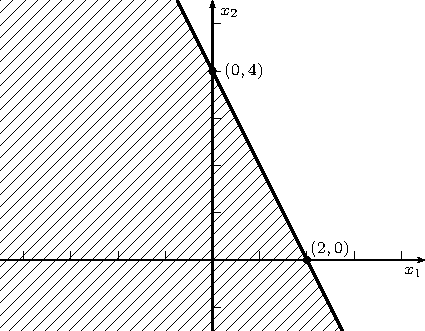
\includegraphics{fig1.pdf}
\end{center}
\end{frame}

\begin{frame}
 \frametitle{Die graphische Methode}
 Hat man es nun mit zwei oder mehr Ungleichungen zu tun, so besteht die Menge aller Punkte $(x_1,x_2)$, die alle diese Ungleichungen erfüllen, aus dem \structure{Durchschnitt der entsprechenden Halbebenen}.

Betrachten wir beispielsweise das LP-Problem
\begin{align}
\begin{alignedat}{4}
\label{eq:1:9}
& \text{maximiere } & x_1 &\ + &\ x_2 & & \\
& \rlap{unter den Nebenbedingungen} & & & & & \\
&& -x_1 &\ + &\ 2x_2 &\ \leq &\  8,\ \\
&& 2x_1 &\ - &\  x_2 &\ \leq &\ 10,\ \\
&& 2x_1 &\ + &\  x_2 &\ \leq &\ 14,\ \\
&& & & \llap{$x_1, x_2$} &\ \geq &\ 0,\ 
\end{alignedat}
\end{align}

so haben wir es bei den Nebenbedingungen mit 5 Ungleichungen zu tun. Die Menge aller $(x_1,x_2)$, die all diese Ungleichungen erfüllen, besteht also aus dem Durchschnitt von fünf Halbebenen:
\end{frame}

\begin{frame}
 \frametitle{Die graphische Methode}
 \begin{center}
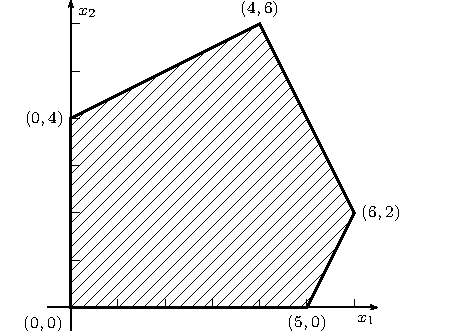
\includegraphics{fig2.pdf}
\end{center}
Wir haben somit den zulässigen Bereich, d.h. die Menge der zulässigen Lösungen von \eqref{eq:1:9}, grafisch dargestellt.
\end{frame}

\begin{frame}
 \frametitle{Einbeziehung der Zielfunktion}
  Nun betrachten wir zusätzlich die Zielfunktion. \\
  \vspace*{0.2cm}
  \textbf{Genauer:} Wir betrachten diejenigen Punkte $(x_1,x_2)$, für die die Zielfunktion den Wert 0 annimmt, für die also gilt:
\[
x_1+x_2 = 0.
\]
Diese Punkte bilden eine Gerade $g$, die mit dem zulässigen Bereich von \eqref{eq:1:9} zumindest einen Punkt gemeinsam hat. Wir sagen, dass die Gerade $g$ den zulässigen Bereich \structure{trifft} oder \structure{schneidet}. Wir nehmen die Gerade $g$ in unsere Zeichnung auf:
\end{frame}

\begin{frame}
 \frametitle{Einbeziehung der Zielfunktion}
 \begin{center}
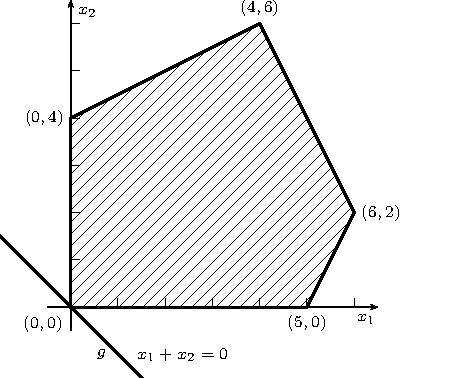
\includegraphics{fig3.pdf}
\end{center}
\end{frame}

\begin{frame}
 \frametitle{Das weitere Vorgehen}
 Betrachten wir für $d \in \R$ die Gleichung
\[
x_1 + x_2 = d,
\]
so wird hierdurch eine zu $g$ parallele Gerade beschrieben. Wählen wir beispielsweise $d=3$, so schneidet diese Gerade den zulässigen Bereich. Das weitere Vorgehen ist nun klar: Man verschiebt die Gerade $g$ parallel und achtet darauf, dass die entstehende Gerade $x_1+x_2=d$ die Menge der zulässigen Lösungen immer noch schneidet, und bemüht sich außerdem, $d$ möglichst groß werden zu lassen.

In unserem Beispiel ergibt sich, dass $d=10$ der größtmögliche Wert ist und dass der Maximalwert $d=10$ im Eckpunkt $(4,6)$ angenommen wird; siehe nachfolgende Zeichnung:
\end{frame}

\begin{frame}
 \frametitle{Das weitere Vorgehen}
 \begin{center}
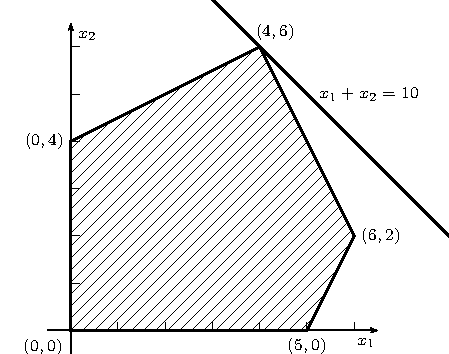
\includegraphics{fig4.pdf}
\end{center}
Der Maximalwert $d = 10$ wird im Eckpunkt $(4, 6)$ angenommen.
\end{frame}

\begin{frame}
 \frametitle{Das Simplexverfahren}
 Betrachte das LP-Problem in \structure{Standardform}:
\begin{align}
\begin{alignedat}{5}
\label{eq:2:1}
& \text{maximiere } & 5x_1 &\ + &\ 4x_2 &\ + &\ 3x_3 & & \\
& \rlap{unter den Nebenbedingungen} & & & & & & & \\
&& 2x_1 &\ + &\ 3x_2 &\ + &\  x_3 &\ \leq &\  5,\ \\
&& 4x_1 &\ + &\  x_2 &\ + &\ 2x_3 &\ \leq &\ 11,\ \\
&& 3x_1 &\ + &\ 4x_2 &\ + &\ 2x_3 &\ \leq &\  8,\ \\
&& & & & & \llap{$x_1, x_2, x_3$} &\ \geq &\  0.\
\end{alignedat}
\end{align}
\end{frame}

\begin{frame}
 \frametitle{Schlupfvariablen}
 Wir führen sogenannte \structure{Schlupfvariablen} ein. \\
 \vspace*{0.2cm}
 \textbf{Beispiel}: erste Nebenbedingung:
\begin{equation}
\label{eq:2:2}
2x_1 + 3x_2 + x_3 \leq 5.
\end{equation}

Ist $(x_1,x_2,x_3)$ eine zulässige Lösung des LP-Problems \eqref{eq:2:1}, so erfüllen die Zahlen $x_1, x_2, x_3$ insbesondere die Ungleichung \eqref{eq:2:2}, wobei es möglich ist, dass $2x_1+3x_2+x_3 < 5$. Die Differenz der rechten und der linken Seite von \eqref{eq:2:2} bezeichnet man als \structure{Schlupf}. Die Differenz zwischen der rechten und der linken Seite von \eqref{eq:2:2} wollen wir $x_4$ nennen; wir \structure{definieren} also:
\[
x_4 := 5 - 2x_1 - 3x_2 - x_3.
\]

Wir können \eqref{eq:2:2} kurz und knapp wie folgt ausdrücken:
\[
x_4 \geq 0.
\]
\end{frame}

\begin{frame}
\frametitle{Schlupfvariablen} 
In ähnlicher Weise definieren wir \structure{Schlupfvariablen}:
\begin{align*}
\begin{alignedat}{5}
x_5 &\ := &\ 11 &\ - &\ 4x_1 &\ - &\  x_2 &\ - &\ 2x_3,\ \\
x_6 &\ := &\  8 &\ - &\ 3x_1 &\ - &\ 4x_2 &\ - &\ 2x_3.\
\end{alignedat}
\end{align*}

Darüber hinaus ist es üblich, noch eine weitere Variable einzuführen, die man mit $z$ bezeichnet und die den Wert der Zielfunktion angibt; in unserem Beispiel:
\[
z = 5x_1 + 4x_2 + 3x_3.
\]
\end{frame}

\begin{frame}
 \frametitle{Neue Variablen: Zusammenfassung}
 Unsere Überlegungen lassen sich wie folgt zusammenfassen: Zu jeder Wahl der Zahlen $x_1,x_2,x_3$ definieren wir die Zahlen $x_4,x_5,x_6$ und $z$, indem wir festlegen:
\begin{align}
\begin{alignedat}{5}
\label{eq:2:3}
x_4 &\ = &\  5 &\ - &\ 2x_1 &\ - &\ 3x_2 &\ - &\  x_3,\ \\
x_5 &\ = &\ 11 &\ - &\ 4x_1 &\ - &\  x_2 &\ - &\ 2x_3,\ \\
x_6 &\ = &\  8 &\ - &\ 3x_1 &\ - &\ 4x_2 &\ - &\ 2x_3,\ \\
z   &\ = &     &    &\ 5x_1 &\ + &\ 4x_2 &\ + &\ 3x_3.\
\end{alignedat}
\end{align}
\end{frame}

\begin{frame}
 \frametitle{Umformulierung}
 Unter Verwendung der Bezeichnungen $x_4,x_5,x_6$ und $z$ aus \eqref{eq:2:3} können wir unser LP-Problem \eqref{eq:2:1} auch wie folgt formulieren:
\begin{align}
\begin{alignedat}{3}
\label{eq:2:4}
& \text{maximiere $z$} & & & \\
& \rlap{unter den Nebenbedingungen} & & &\\
&& x_1,x_2,x_3,x_4,x_5,x_6 &\ \geq &\ 0.
\end{alignedat}
\end{align}

Bei \eqref{eq:2:4} handelt es sich nur um eine \alert{Umformulierung} von \eqref{eq:2:1}, wobei die Bezeichnungen $x_4$, $x_5$, $x_6$ und $z$ aus \eqref{eq:2:3} verwendet werden. Es gilt:
\begin{enumerate}[1.]
\item Jede zulässige Lösung $(x_1,x_2,x_3)$ von \eqref{eq:2:1} kann auf eindeutige Art zu einer zulässigen Lösung von \eqref{eq:2:4} erweitert werden, indem man $x_1$, $x_2$ und $x_3$ in \eqref{eq:2:3} einsetzt.
\item Ist umgekehrt $(x_1,x_2,x_3,x_4,x_5,x_6)$ eine zulässige Lösung von \eqref{eq:2:4}, wobei $x_4$, $x_5$ und $x_6$ die in \eqref{eq:2:3} angegebene Bedeutung haben, so kann man auf eine sehr einfache Art eine zulässige Lösung $(x_1,x_2,x_3)$ von \eqref{eq:2:1} erhalten: Man braucht die Schlupfvariablen $x_4,x_5,x_6$ nur wegzulassen.
\end{enumerate}
\end{frame}

\begin{frame}
 \frametitle{Grundidee des Simplexverfahrens}
 Wir führen nun vor, wie man mithilfe des Simplexverfahrens eine optimale Lösung von \eqref{eq:2:1} bzw. \eqref{eq:2:4} findet. \\
 \vspace*{0.2cm}
 \textbf{Grundidee:} Man versucht zulässige Lösungen schrittweise zu verbessern, mit dem Ziel, nach endlich vielen Schritten bei einer optimalen Lösung anzukommen. \\
 \textbf{Mit anderen Worten}: Wenn wir eine zulässige Lösung $(x_1,\ldots,x_6)$ von \eqref{eq:2:4} haben, so versuchen wir eine zulässige Lösung $(x_1',\ldots,x_6')$ von \eqref{eq:2:4} zu finden, für die gilt:
 \[
 5 x_1' + 4x_2' + 3 x_3' > 5x_1 + 4x_2 + 3x_3.
 \]
\end{frame}

\begin{frame}
 \frametitle{Zul\"assige Startl\"osung}
 Damit dieser Prozess in Gang kommt, braucht man natürlich eine zulässige \structure{Startlösung}, in unserem Beispiel z.B. $x_1=x_2=x_3=0$.

Mithilfe von \eqref{eq:2:3} erhält man dann dazugehörige Werte für $x_4$, $x_5$ und $x_6$:
\[
x_4 = 5, \qquad x_5 = 11, \qquad x_6 = 8.
\]
Unsere Startlösung lautet also:
\begin{equation}
\label{eq:2:5}
x_1=0, \quad x_2=0, \quad x_3=0, \quad x_4 = 5, \quad x_5 = 11, \quad x_6 = 8.
\end{equation}

Hierbei handelt es sich in der Tat um eine \structure{zulässige Lösung} von \eqref{eq:2:4}, da $x_1, \ldots, x_6$ so gewählt wurden, dass \eqref{eq:2:3} gilt, und da außerdem die Bedingungen $x_1,\ldots, x_6 \geq 0$ erfüllt sind.

Den zu dieser Lösung dazugehörigen \structure{Zielfunktionswert} $z$ erhalten wir indem wir in \eqref{eq:2:3} für $x_1,x_2,x_3$ den Wert $0$ einsetzen. Man erhält
\[
z=0.
\]
\end{frame}

\begin{frame}
 \frametitle{Verbesserung der Startlösung (Beginn der 1. Iteration)}
 \alert{Wir versuchen nun eine zulässige Lösung mit einem höheren Zielfunktionswert $z$ finden!} \\
 \vspace*{0.2cm}
 Lassen wir beispielsweise die Werte für $x_2$ und $x_3$ unverändert bei $x_2=x_3=0$ und vergrößern $x_1$, so erhalten wir
 \[
 z = 5x_1 > 0.
 \]
 Z.B. für $x_2=x_3=0$ und $x_1=1$ erhalten wir die zulässige Lösung
 \[
 x_1=1, \quad x_2=0, \quad x_3=0, \quad x_4=3, \quad x_5=7, \quad x_6=5 \quad \text{mit} \quad z=5.
 \]
 %Wählen wir $x_1=2$ und nach wie vor $x_2=x_3=0$, so erhalten wir einen noch besseren Zielfunktionswert: $z=10$. Außerdem gilt $x_4=1$, $x_5=3$, $x_6=2$.
 Versuchen wir dasselbe mit $x_1=3$ und $x_2=x_3=0$, so erhalten wir $z=15$, was ein noch besserer Zielfunktionswert wäre. Aber gleichzeitig erhalten wir auch $x_4 = -1$. \alert{Das bedeutet, dass wir den Bereich der zulässigen Lösungen verlassen haben}: Es muss ja immer $x_4 \geq 0$, $x_5 \geq 0$ und $x_6 \geq 0$ gelten. Wir haben $x_1$ also zu stark erhöht.
\end{frame}

\begin{frame}
 \frametitle{Verbesserung der Startlösung (Beginn der 1. Iteration)} 
 \textbf{Frage:} Um wie viel können wir $x_1$ maximal erhöhen (unter Beibehaltung von $x_2=x_3=0$), ohne dass einer der Werte $x_4, x_5, x_6$ negativ wird?

 \textbf{Antwort:} Da $x_2=x_3=0$ gelten soll, haben wir
\begin{align*}
 \begin{alignedat}{3}
 x_4 &\ = &\  5 &\ - &\ 2x_1,\ \\
 x_5 &\ = &\ 11 &\ - &\ 4x_1,\ \\
 x_6 &\ = &\  8 &\ - &\ 3x_1.\
 \end{alignedat}
\end{align*}
Wir sehen also:
\begin{align*}
  x_4 \ge 0 \quad \Leftrightarrow \quad x_1 \leq \frac{5}{2}, \quad
  x_5 \ge 0 \quad \Leftrightarrow \quad x_1 \leq \frac{11}{4}, \quad
  x_6 \ge 0 \quad \Leftrightarrow \quad x_1 \leq \frac{8}{3}.
\end{align*}
 Die erste Bedingung schränkt $x_1$ am stärksten ein; wir wählen also $x_1 = \frac{5}{2}$ und erhalten somit die zulässige Lösung
\begin{equation}
\label{eq:2:6}
x_1=\frac{5}{2}, \qquad x_2=0, \qquad x_3=0, \qquad x_4=0, \qquad  x_5=1, \qquad x_6=\frac{1}{2}.
\end{equation}

Als verbesserten Zielfunktionswert erhalten wir \alert{$z = \frac{25}{2}$.} Dieses Ergebnis wollen wir nun noch weiter verbessern!
\end{frame}

\begin{frame}
 \frametitle{Fortführung der 1. Iteration}
 Die entscheidende Rolle in der 1. Iteration spielte das Gleichungssystem \eqref{eq:2:3}: Dort wurden die vier Variablen $x_4,x_5,x_6$ und $z$ durch die drei übrigen Variablen (nämlich durch $x_1,x_2,x_3$) dargestellt und diese drei Variablen besaßen alle den Wert Null in unserer Startlösung.

Diesen Zustand wollen wir nun (bezogen auf die verbesserte Lösung \eqref{eq:2:6} wiederherstellen. In \eqref{eq:2:6} sind $x_2, x_3$ und $x_4$ diejenigen Variablen, die den Wert Null annehmen. Diese Variablen sollen nun die Rolle spielen, die zuvor von $x_1$, $x_2$ und $x_3$ gespielt wurde. Hierzu formen wir \eqref{eq:2:3} so um, dass auf der linken Seite nun $x_1$, $x_5$, $x_6$ und $z$ stehen, während rechts nur noch $x_2$, $x_3$ und $x_4$ auftauchen.\\
\vspace*{0.2cm}
\textbf{Anders gesagt:} $x_1$ und $x_4$ sollen ihre Rollen tauschen.
\end{frame}

\begin{frame}
\frametitle{Rollentausch von $x_1$ und $x_4$}
 Hierzu formen wir zunächst diejenige Zeile von \eqref{eq:2:3} um, in der $x_4$ auf der linken Seite steht. In \eqref{eq:2:3} ist das die erste Zeile; wir erhalten
\begin{equation}
\label{eq:2:7}
x_1 = \frac{5}{2} - \frac{3}{2}x_2 - \frac{1}{2}x_3 - \frac{1}{2}x_4.
\end{equation}

Einsetzen von \eqref{eq:2:7} in die übrigen Zeilen von \eqref{eq:2:3} ergibt:
\begin{align*}
x_5 &= 11 - 4 \cdot \left( \frac{5}{2} - \frac{3}{2}x_2 - \frac{1}{2}x_3 - \frac{1}{2}x_4 \right) - x_2 - 2x_3 \\
    &= 1 + 5x_2 + 2x_4, \\
x_6 &= 8 - 3 \cdot \left( \frac{5}{2} - \frac{3}{2}x_2 - \frac{1}{2}x_3 - \frac{1}{2}x_4 \right) -4x_2 - 2x_3 \\
    &= \frac{1}{2} + \frac{1}{2}x_2 - \frac{1}{2}x_3 + \frac{3}{2}x_4, \\
z   &= 5 \cdot \left( \frac{5}{2} - \frac{3}{2}x_2 - \frac{1}{2}x_3 - \frac{1}{2}x_4 \right) + 4x_2 + 3x_3 \\
    &= \frac{25}{2} - \frac{7}{2}x_2 + \frac{1}{2}x_3 - \frac{5}{2}x_4.
\end{align*}
\end{frame}

\begin{frame}
 \frametitle{Ergebnis der 1. Iteration}
 Also lautet unser neues, durch Umformung von \eqref{eq:2:3} entstandenes Gleichungssystem:
\begin{align}
\begin{alignedat}{5}
\label{eq:2:8}
x_1 &\ = &\  \frac{5}{2} &\ - &\ \frac{3}{2}x_2 &\ - &\ \frac{1}{2}x_3 &\ - &\ \frac{1}{2}x_4,\ \\
x_5 &\ = &\            1 &\ + &\           5x_2 &    &                 &\ + &\           2x_4,\ \\
x_6 &\ = &\  \frac{1}{2} &\ + &\ \frac{1}{2}x_2 &\ - &\ \frac{1}{2}x_3 &\ + &\ \frac{3}{2}x_4,\ \\
z   &\ = &\ \frac{25}{2} &\ - &\ \frac{7}{2}x_2 &\ + &\ \frac{1}{2}x_3 &\ - &\ \frac{5}{2}x_4.\
\end{alignedat}
\end{align}

Analog zur 1. Iteration versuchen wir nun, den aktuellen Wert von $z$ zu vergrößern, indem wir den Wert einer der drei Variablen auf der rechten Seite von (\ref{eq:2:8}) anheben, während wir gleichzeitig die beiden anderen Variablen der rechten Seite bei Null lassen.\\
\vspace*{0.2cm}
\textbf{Drei M\"oglichkeiten}:
\begin{enumerate}[(i)]
\item $x_2$ wird angehoben, $x_3=x_4=0$ (verkleinert aber $z$);
\item $x_3$ wird angehoben, $x_2=x_4=0$;
\item $x_4$ wird angehoben, $x_2=x_3=0$ (verkleinert aber $z$).
\end{enumerate}
\end{frame}

\begin{frame}
 \frametitle{Anhebung von $x_3$}
 \alert{Es bleibt nur eine Wahl:} Wir setzen $x_2=x_4=0$ und versuchen durch Anheben von $x_3$ zu einem möglichst großen Zuwachs von $z$ zu gelangen, wobei wir allerdings darauf achten müssen, dass weiterhin $x_1 \geq 0$, $x_5 \geq 0$ und $x_6 \geq 0$ gilt. \\ \vspace*{0.2cm}
 \textbf{Wie stark können wir $x_3$ anheben}? Aus \eqref{eq:2:8} lesen wir ab: Wegen $x_2=x_4=0$ ist die Bedingung $x_1 \geq 0$ äquivalent zu $\frac{5}{2} - \frac{1}{2}x_3 \geq 0$, woraus man $x_3 \leq 5$ erhält. Analog: 
 \begin{equation*}
  x_6 \geq 0 \quad \Leftrightarrow \quad x_3 \leq 1, \quad x_5 \geq 0 \quad \Leftrightarrow \quad x_3 \text{ beliebig}
 \end{equation*}
 \textbf{Also}: $x_3=1$ ist das Beste, was wir erreichen können, und unsere neue Lösung ist dementsprechend:
\begin{equation}
\label{eq:2:9}
x_1=2, \quad x_2=0, \quad x_3=1, \quad x_4=0, \quad x_5=1, \quad x_6=0.
\end{equation}
\end{frame}

\begin{frame}
 \frametitle{Austausch von $x_3$ und $x_6$}
 \textbf{Wir wissen bereits:} Damit das Verfahren weitergeht, brauchen wir nicht nur eine verbesserte Lösung, sondern auch eine neue Darstellung unseres Gleichungssystems \eqref{eq:2:8}, die zu \eqref{eq:2:9} passt. In \eqref{eq:2:9} gibt es drei Variablen, die den Wert Null annehmen: $x_2=x_4=x_6=0$. Diese sollen nun auf der rechten Seite stehen, die übrigen Variablen ($x_1,x_3,x_5$ sowie $z$) sollen links auftauchen: Wir müssen $x_3$ und $x_6$ austauschen. Dementsprechend stellen wir die dritte Gleichung von \eqref{eq:2:8} um und erhalten
\[
x_3 = 1 + x_2 + 3x_4 - 2x_6.
\]

Setzt man dies für $x_3$ in die übrigen Gleichungen von \eqref{eq:2:8} ein, so erhält man
\begin{align}
\begin{alignedat}{5}
\label{eq:2:10}
x_3 &\ = &\  1 &\ + &\  x_2 &\ + &\ 3x_4 &\ - &\ 2x_6,\ \\
x_1 &\ = &\  2 &\ - &\ 2x_2 &\ - &\ 2x_4 &\ + &\  x_6,\ \\
x_5 &\ = &\  1 &\ + &\ 5x_2 &\ + &\ 2x_4, &    &        \\
z   &\ = &\ 13 &\ - &\ 3x_2 &\ - &\  x_4 &\ - &\  x_6.\
\end{alignedat}
\end{align}

Einsetzen von $x_2=x_4=x_6=0$ in die letzten Zeile von \eqref{eq:2:10} ergibt $z=13$.
\end{frame}

\begin{frame}
  \frametitle{Die 3. Iteration -- Wir sind fertig!}
  \alert{Bei der dritten Iteration stecken wir fest}. Dies entpuppt sich allerdings als \alert{Erfolg:} Die Lösung \eqref{eq:2:9} ist optimal, der Zielfunktionswert $z=13$ ist bestmöglich. \\ \vspace*{0.2cm} 
  \textbf{Weshalb ist das so?} Die Antwort findet sich in der letzten Zeile von \eqref{eq:2:10}:
\begin{equation} \label{eq:2:11}
z = 13 - 3x_2 - x_4 - x_6.
\end{equation}
Unsere letzte Lösung \eqref{eq:2:9} hat zu $z=13$ geführt.  Es ist aber klar: Ist $(x_1,x_2,x_3,x_4,x_5,x_6)$ eine beliebige zulässige Lösung, so gilt insbesondere $x_2 \geq 0$, $x_4 \geq 0$ und $x_6 \geq 0$, woraus sich (aufgrund von \eqref{eq:2:11}) $z \leq 13$ ergibt.
\end{frame}

\end{document}
